\documentclass[12pt,a4paper]{report}

% Packages
\usepackage[spanish]{babel} % Set language to Spanish
\usepackage{graphicx}
\usepackage{amsmath}
\usepackage{hyperref}
\usepackage{setspace}
\usepackage{float}

% Title and Author (adjust the spacing as needed)
\title{\LARGE \textbf{PROJECT TITLE}}
\author{}
\date{\large On: \today}

% Begin Document
\begin{document}

% Title Page
\makeatletter
\begin{titlepage}
    \centering
    \vspace*{1cm}
    
    {\LARGE \textbf{Propuesta Caso de Uso:}}\\[0.65cm]
    {\LARGE \textbf{Air Quality Monitoring using}}\\
    {\LARGE \textbf{ Web Scraping \& AWS Services}}\\[1cm]

    { 
\includegraphics[width=12cm]{img.png}}\\[1cm]
    
   \textbf{Sistemas y Servicios en la Nube}\\
    
    Máster Universitario en Ingeniería Informática\\[1.5cm]
    
    \textbf{Manuel Brazález Cañadas}\\
    manuel.brazalez@alu.uclm.es\\
    \textbf{Abel Ortiz Villaescusa}\\
    abel.ortiz1@alu.uclm.es\\
    \textbf{Álvaro Mayorga Zarco}\\
    alvaro.mayorga@alu.uclm.es\\[2cm]
    \date{\large \today}
    {\@date\\}
\end{titlepage}
\makeatother

% Table of Contents
\tableofcontents

% List of Figures
\listoffigures

\newpage

\section*{1. Propuesta del Caso de Uso}
\addcontentsline{toc}{chapter}{1. Propuesta del Caso de Uso} % Adds it to the ToC manually

Nuestro objetivo en este proyecto será crear una arquitectura en AWS capaz de recolectar información relacionada con la
calidad del aire a través del uso de web scraping. Para ello, utilizaremos la página web \href{https://troposfera.es/datos/dev-albacete/#/dashboard}{troposfera.es} como fuente de datos.
En base a los datos recopilados, podremos monitorizar la calidad del aire en la ciudad de Albacete con el objetivo
de estudiar la calidad del aire en tiempo real y poder tomar decisiones en base a esta información.
\newline
En la figura \ref{fig:diagrama}, se muestra la arquitectura propuesta junto con los puntos claves de la misma que se detallan a continuación:
\begin{itemize}%[leftmargin=*]
    \item \textbf{Paso 1.} Definiremos cada cuánto queremos que se ejecute la lambda que se encargará del webscraping usando un schedule event.
    \item \textbf{Paso 2.} Utilizaremos el servicio de AWS EventBridge con el schedule previamente configurado, para programar la ejecución de la función lambda que contiene el código para realizar el web scraping que se encargará de recopilar los datos de la página web mencionada anteriormente.
    \item \textbf{Paso 3.} Los datos recopilados se almacenarán en una base de datos NoSQL de AWS DynamoDB.
    \item \textbf{Paso 4.} Con la ayuda del servicio de AWS QuickSight podremos ofrecer a un usuario los datos almacenados en DynamoDB de una forma visual y sencilla.
    \item \textbf{Paso 5.} Al añadir un nuevo dato a la base de datos, se disparará una lambda encargada de enviar una notificación a un usuario a través del servicio de mensajería SNS.
    \item \textbf{Paso 6.} La función lambda que se encarga de enviar la notificación al tópico de SNS, para que los usuarios suscritos reciban un email indicando que se ha almacenado en la base de datos
    nueva información relacionada con la calidad del aire.
\end{itemize}

\begin{figure}[H]
    \centering
    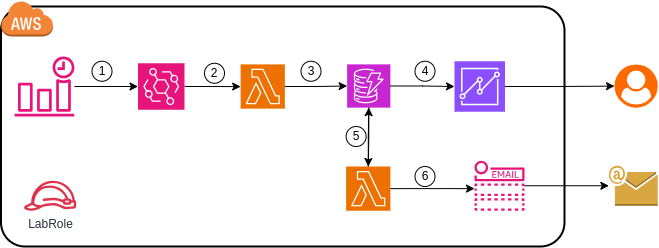
\includegraphics[width=1\textwidth]{diagrama.png}
    \caption{Diagrama de la arquitectura propuesta}
    \label{fig:diagrama}
\end{figure}


\end{document}